\capitulo{SISTEMA DESENVOLVIDO}

\secao{Modelo Tratado}

\secao{Proposta de Solução}

Será desenvolvido um sistema que otimiza a alocação das salas em até 90\% facilizando a vida do gerente.Por se tratar de um problema especifico fica dificil encontrar tecnoloagias disponiveis para a resolução do problema sendo assim necessario o atendimento de um sistema que atenda todas as necessisdades exigidas.

\secao{O Sistema Desenvolvido}
	
	Descrição sobre o Sistema

\subsecao{Ambiente de Desenvolvimento}

	IDE eclipse, sublimeText, Google Chrome, programa DIA para o desenvolvimento dos diagramas\cite{alterar}

\subsecao{Modegem do Sistema}

	Antes de tudo foi necessaria a modelagem do sistema, para que todos os requisitos fossem atendidos de acordo com a necessidade.\par

	Achar alguma referencia sobre metodologias de modelagem de dados UML\par\cite{alterar}

	Para a analise deste sistema foram desenvolvidos os seguintes diagramas:\par\cite{alterar}
	
	Diagramas de Caso de Uso\par
	Diagramas de classes\par
	Diagramas de Seqüência\par
	Diagrama de Atividades\par
	Diagrama de Estados\par
\begin{figure}[!htb]
   \caption[Diagrama de componetes do sistema xxx]{Diagrama de componetes do sistema xxx}
   \label{fig:figura1}
   \centering
   \includegraphics{images/diagramaComponentes.png}
   \\ \textbf{\footnotesize Fonte: Desenvolvido pelo autor}
\end{figure}


\subsecao{Diagrama de Caso de Uso: Sistema}


	Criar o caso de uso que diz respeito a todas as funcionalidades que o sistema tem de cadastro e manutenção.\par\cite{alterar}

	Caso de uso do sistema\par\cite{alterar}

	\begin{figure}[!htb]
		\centering
   		\caption[Diagrama de caso de uso]{Diagrama de caso de uso}
   		\label{fig:figura2}
   		\centering
   		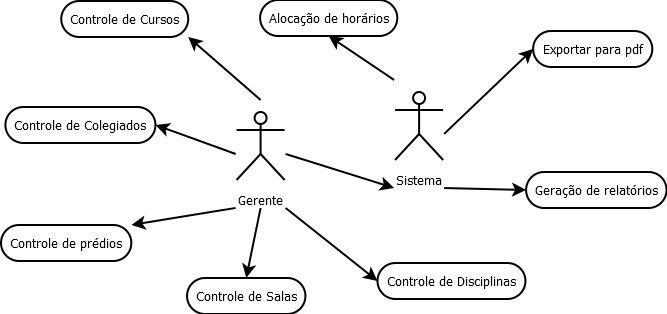
\includegraphics[scale=0.5]{diagramaCasoUso.png}
   		\\ \textbf{\footnotesize Fonte: Autor}
	\end{figure}


\subsubsecao{Diagrama de Atividade: Alocação}
	
	Descrever a rotina de atividades da alocação do sistema
	

\subsubsecao{Diagrama de Classe das controllers}
		
	Achar alguma referencia de diagrama de classe.

	Imagem do diagrama de classe das controllers

\subsubsecao{Diagrama de Classe das models}
	
	Imagem do diagrama de classe das models

\subsubsecao{Diagrama de Classe das views}
	
	Imagem do diagrama de classe das views

\subsubsecao{Modelagem de Dados}

	Achar alguma referencia de modelagem de dados

	Inserir imagem do modelo

		\begin{figure}[!htb]
   		\caption[Modelagem Banco de Dados]{Modelagem Banco de Dados}
   		\label{fig:figura3}
   		\centering
   		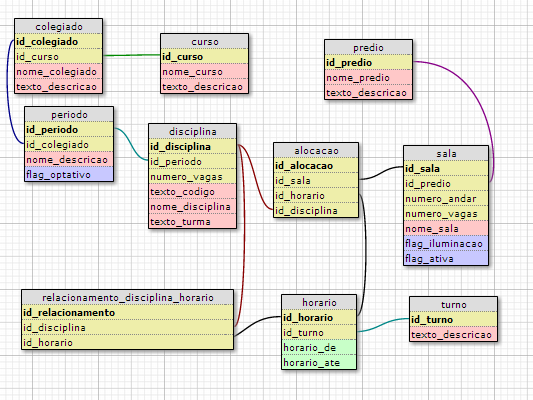
\includegraphics{modelagemBanco.png}
   		\\ \textbf{\footnotesize Fonte: Autor}
	\end{figure}

\subsecao{Funcionalidades}

	O sistema consiste nas seguintes funcionalidades.

	1. Controle de cursos \par
	2. Controle de colegiados\par
	3. Controle de disciplinas\par
	4. Controle de salas\par
	5. Controle de prédios\par
	6. Alocação de horários\par
	7. Geração de relatórios\par
	8. Exportar para pdf\par



\subsecao{Dados de Entrada}

	Como serão inseriadas as informações, e quais são os dados de entrada

	Informados pelo gerente.

\subsecao{Alocação}

	Processa os dados de alocação

\subsecao{Relatórios}

	Geração dos relatorios determinados na analise do sistema, todos os relatorios podem ser exportados para pdf
